\documentclass{article}
\usepackage[left=0.5in,top=0.5in,right=0.5in,bottom=0.5in]{geometry}
\usepackage[english]{babel}
\usepackage[utf8]{inputenc}
\usepackage[table]{xcolor}
\usepackage{amssymb,amsmath,amsthm}
\usepackage{changepage,threeparttable}
\usepackage{booktabs,multirow}
\usepackage{graphicx}
\usepackage{soul}
\graphicspath{{./images/}}
\def\F#1{\(#1\)}
\title{Lab 9: RC Discharge}
\author{Philip Kim}
\date{\today}
\begin{document}
\maketitle
\vspace*{-1cm}
\begin{table}[!htp]\centering
  \begin{tabular}{|c|c|c|c|c|c|c|c|c|c|c|}\hline
    \multicolumn{11}{|c|}{\textbf{Table 1: Discharge}} \\\hline
    \F{R}&\F{C}&\F{f (Hz)}&\F{V_{min} (V)}&\F{t_{srn} (DIV)}&\F{SEC/DIV}&\F{t_{srn} (s)}&\F{V_{srn} (DIV)}&\F{V/DIV}&\F{V_{srn}} (V)&\F{V_{dischg} (V)}\\\hline
% height = 0.2V/DIV
% width = 50us/DIV
% R = 100 Ohms
% C = 0.22 microfarad

% V_min (V) = 0.2V/DIV
% = 0.2/3
% = .0666/2
% = .0333

% left/right
% t_screen (DIV) = +/- 2.3

% t_screen (s) = 50us/DIV
% = 50/3
% = 16.666667/2
% = 8.333334

% up/down
% V_screen (DIV) = +/- 3

% V_screen (V) = 0.61 - (-0.60)
% = 1.21

% V_discharge (V) = V_screen (V) - V_min (V)
% = 1.21 - .0333
% = 1.1767

% Vmax=0.65;
% Vmin=-0.66;

% V_screenDIV=3.1;% vertical
% t_screenDIV=4.4;% hortizontal

% V_minV=0.2/V_screenDIV;% vertical
% t_screenS=50/t_screenDIV;% hortizontal

% V_screenV=Vmax-Vmin;
% V_dischargeV=V_screenV-V_minV;

    \F{100\Omega}&\F{0.22\mu{F}}&4.024kHz&0.067&\F{\pm}4.00&50us&12.50&\F{\pm}3.0&0.2V&1.20&1.13\\\hline
    \F{100\Omega}&\F{0.22\mu{F}}&4.024kHz&0.065&\F{\pm}4.40&50us&11.36&\F{\pm}3.1&0.2V&1.36&1.29\\\hline
    \F{100\Omega}&\F{0.22\mu{F}}&4.024kHz&0.061&\F{\pm}5.00&50us&10.00&\F{\pm}3.3&0.2V&1.46&1.40\\\hline
    \F{100\Omega}&\F{0.22\mu{F}}&4.024kHz&0.050&\F{\pm}5.10&50us&9.80&\F{\pm}4.0&0.2V&1.54&1.49\\\hline
    \F{100\Omega}&\F{0.22\mu{F}}&4.024kHz&0.048&\F{\pm}5.20&50us&9.62&\F{\pm}4.2&0.2V&1.66&1.61\\\hline

    \F{150\Omega}&\F{0.22\mu{F}}&3.024kHz&0.067&\F{\pm}6.40&50us&7.81&\F{\pm}3.0&0.2V&1.19&1.12\\\hline
    \F{150\Omega}&\F{0.22\mu{F}}&3.024kHz&0.065&\F{\pm}6.45&50us&7.75&\F{\pm}3.1&0.2V&1.27&1.21\\\hline
    \F{150\Omega}&\F{0.22\mu{F}}&3.024kHz&0.063&\F{\pm}6.31&50us&7.64&\F{\pm}3.2&0.2V&1.35&1.29\\\hline
    \F{150\Omega}&\F{0.22\mu{F}}&3.024kHz&0.058&\F{\pm}6.30&50us&7.34&\F{\pm}3.4&0.2V&1.44&1.38\\\hline
    \F{150\Omega}&\F{0.22\mu{F}}&3.024kHz&0.050&\F{\pm}6.25&50us&6.00&\F{\pm}4.0&0.2V&1.52&1.47\\\hline

    \F{270\Omega}&\F{0.22\mu{F}}&2.024kHz&0.067&\F{\pm}9.40&50us&5.42&\F{\pm}3.0&0.2V&1.20&1.13\\\hline
    \F{270\Omega}&\F{0.22\mu{F}}&2.024kHz&0.065&\F{\pm}9.30&50us&5.38&\F{\pm}3.1&0.2V&1.26&1.20\\\hline
    \F{270\Omega}&\F{0.22\mu{F}}&2.024kHz&0.063&\F{\pm}9.20&50us&5.26&\F{\pm}3.2&0.2V&1.35&1.29\\\hline
    \F{270\Omega}&\F{0.22\mu{F}}&2.024kHz&0.059&\F{\pm}9.10&50us&5.16&\F{\pm}3.3&0.2V&1.41&1.35\\\hline
    \F{270\Omega}&\F{0.22\mu{F}}&2.024kHz&0.050&\F{\pm}8.90&50us&5.00&\F{\pm}4.0&0.2V&1.52&1.47\\\hline

    \F{47\Omega}&\F{0.22\mu{F}}&8.024kHz&0.067&\F{\pm}2.20&50us&22.73&\F{\pm}3.0&0.2V&1.20&1.13\\\hline
    \F{47\Omega}&\F{0.22\mu{F}}&8.024kHz&0.063&\F{\pm}2.40&50us&20.63&\F{\pm}3.2&0.2V&1.29&1.23\\\hline
    \F{47\Omega}&\F{0.22\mu{F}}&8.024kHz&0.061&\F{\pm}2.45&50us&20.41&\F{\pm}3.3&0.2V&1.38&1.32\\\hline
    \F{47\Omega}&\F{0.22\mu{F}}&8.024kHz&0.059&\F{\pm}2.50&50us&20.20&\F{\pm}3.4&0.2V&1.46&1.40\\\hline
    \F{47\Omega}&\F{0.22\mu{F}}&8.024kHz&0.050&\F{\pm}2.50&50us&19.83&\F{\pm}4.0&0.2V&1.54&1.49\\\hline
  \end{tabular}
\end{table}
\begin{center}
  \subsection*{Setup}
  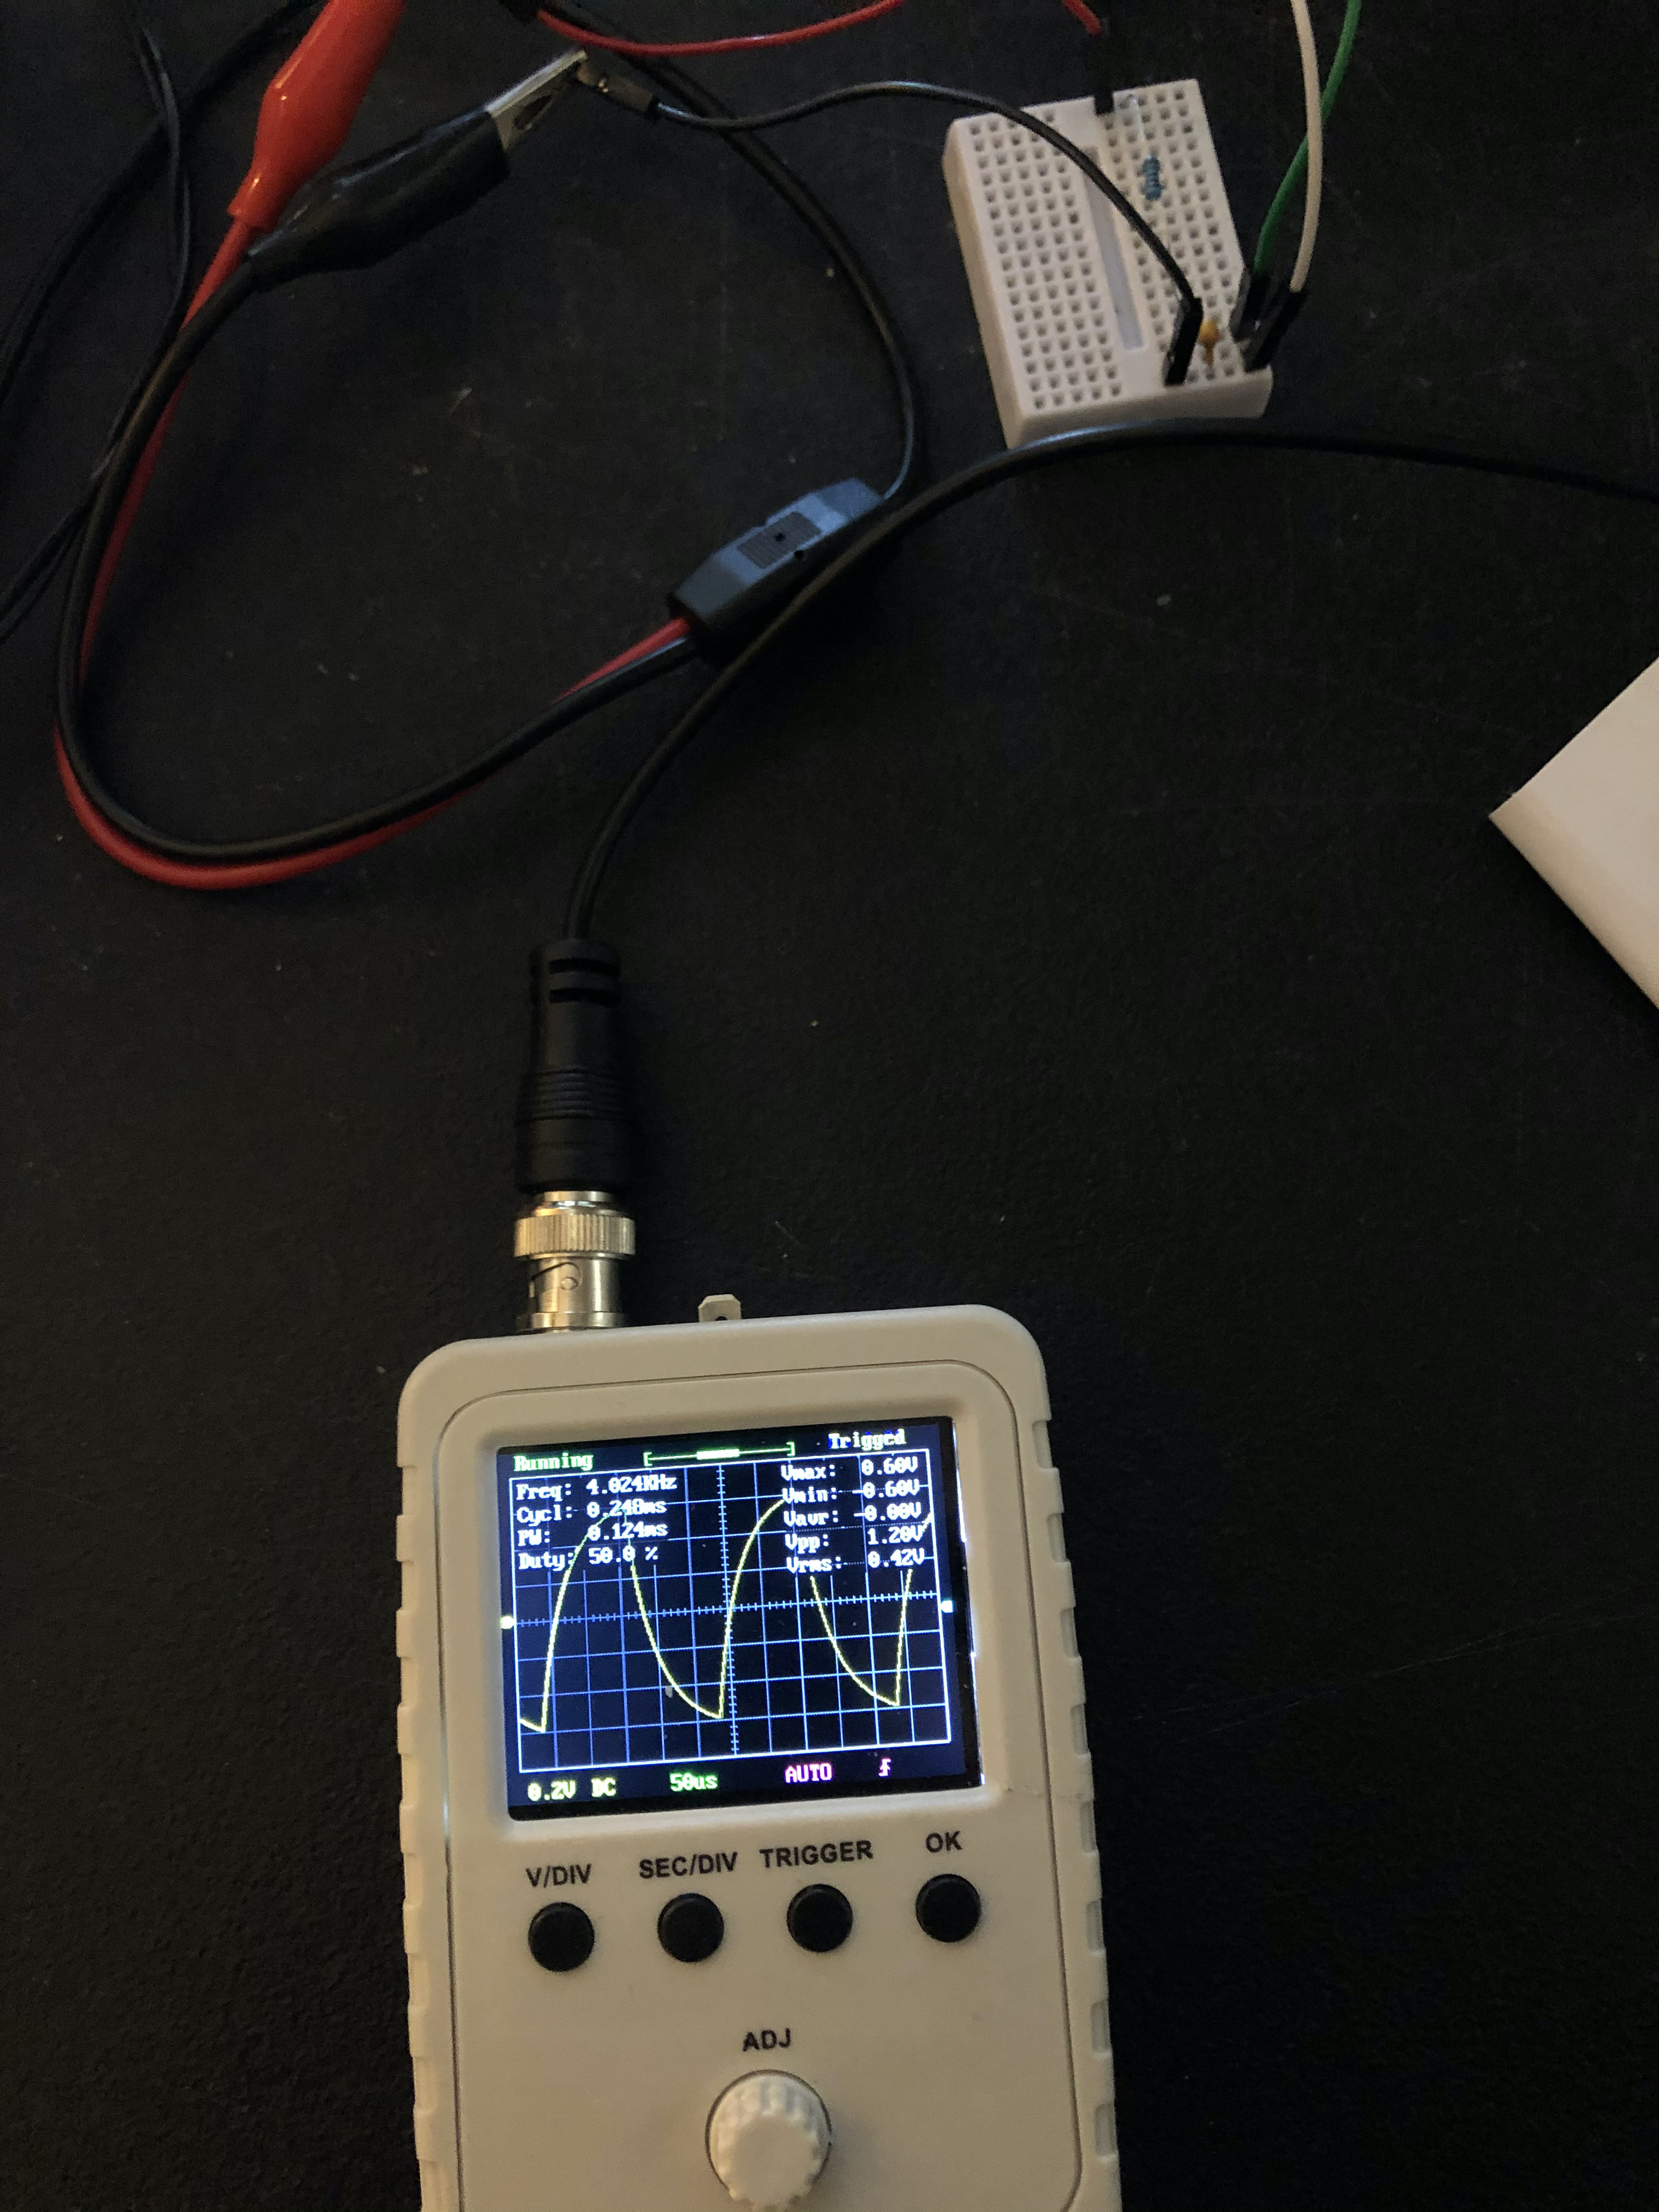
\includegraphics[scale=0.07]{setup.jpeg}
\end{center}
\begin{center}
  \subsection*{Graph 1}
  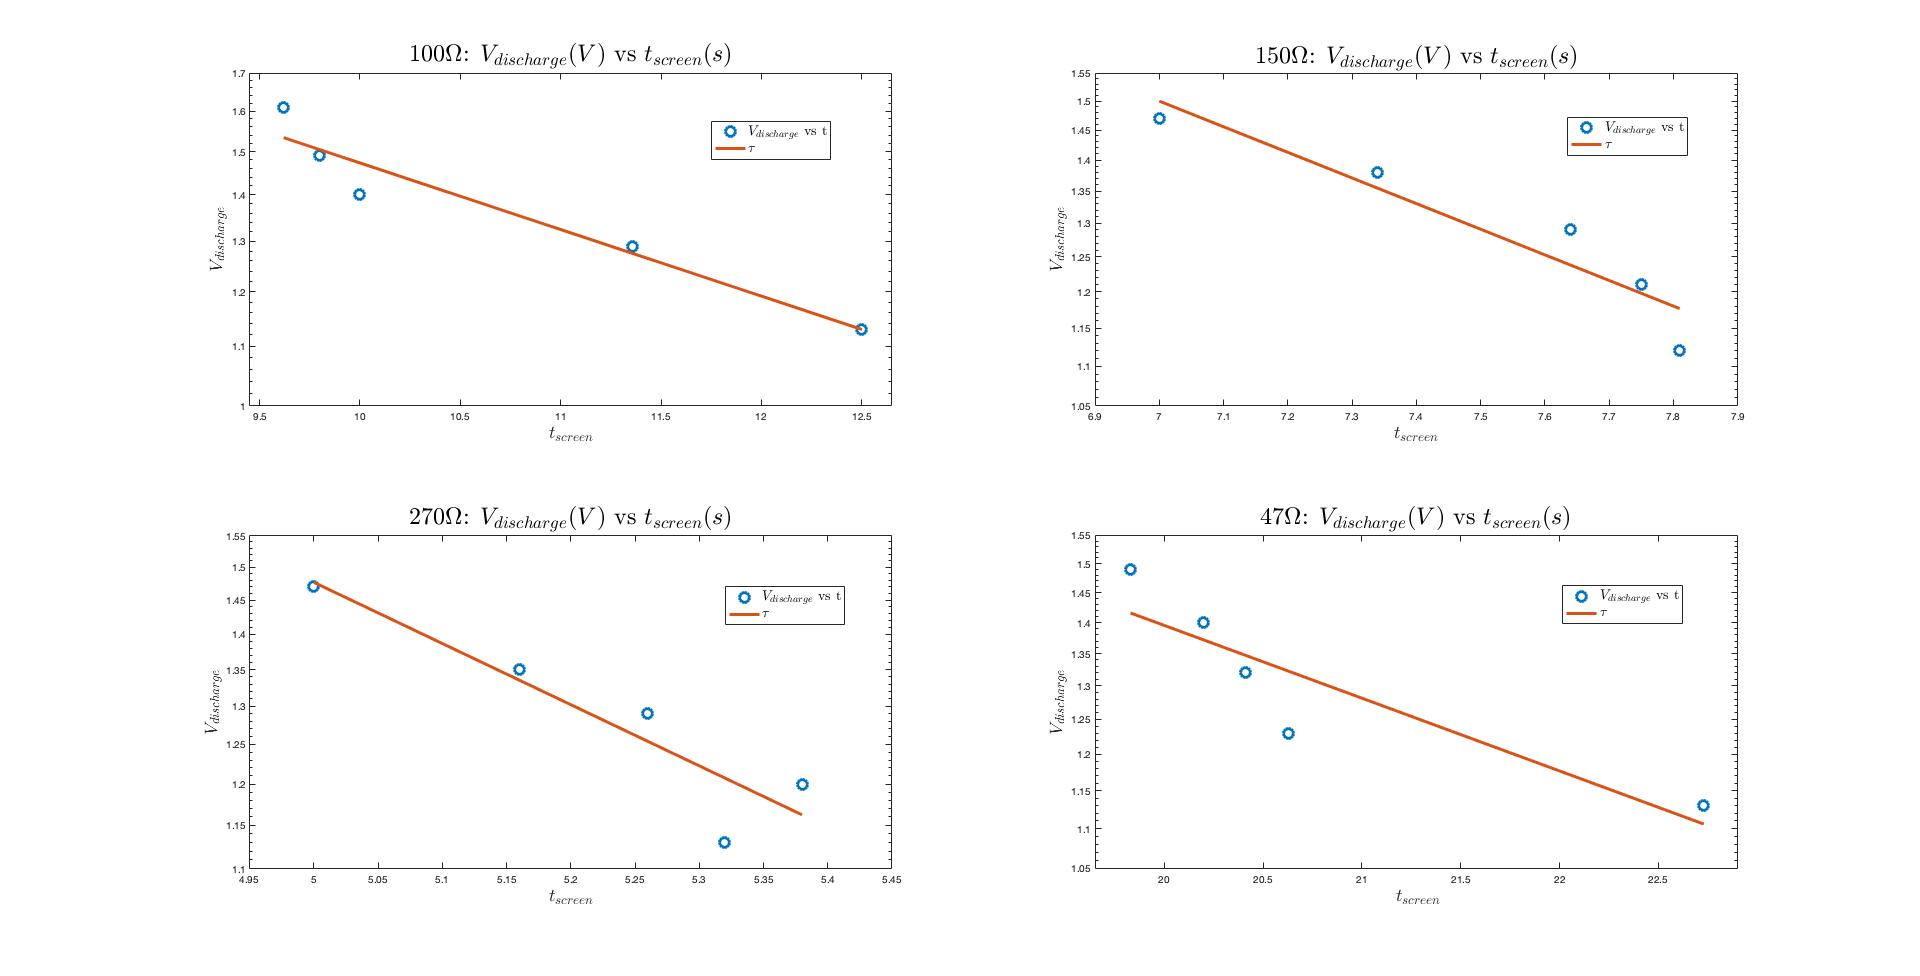
\includegraphics[width=\textwidth]{graph1.jpg}
  \subsection*{Graph 2}
  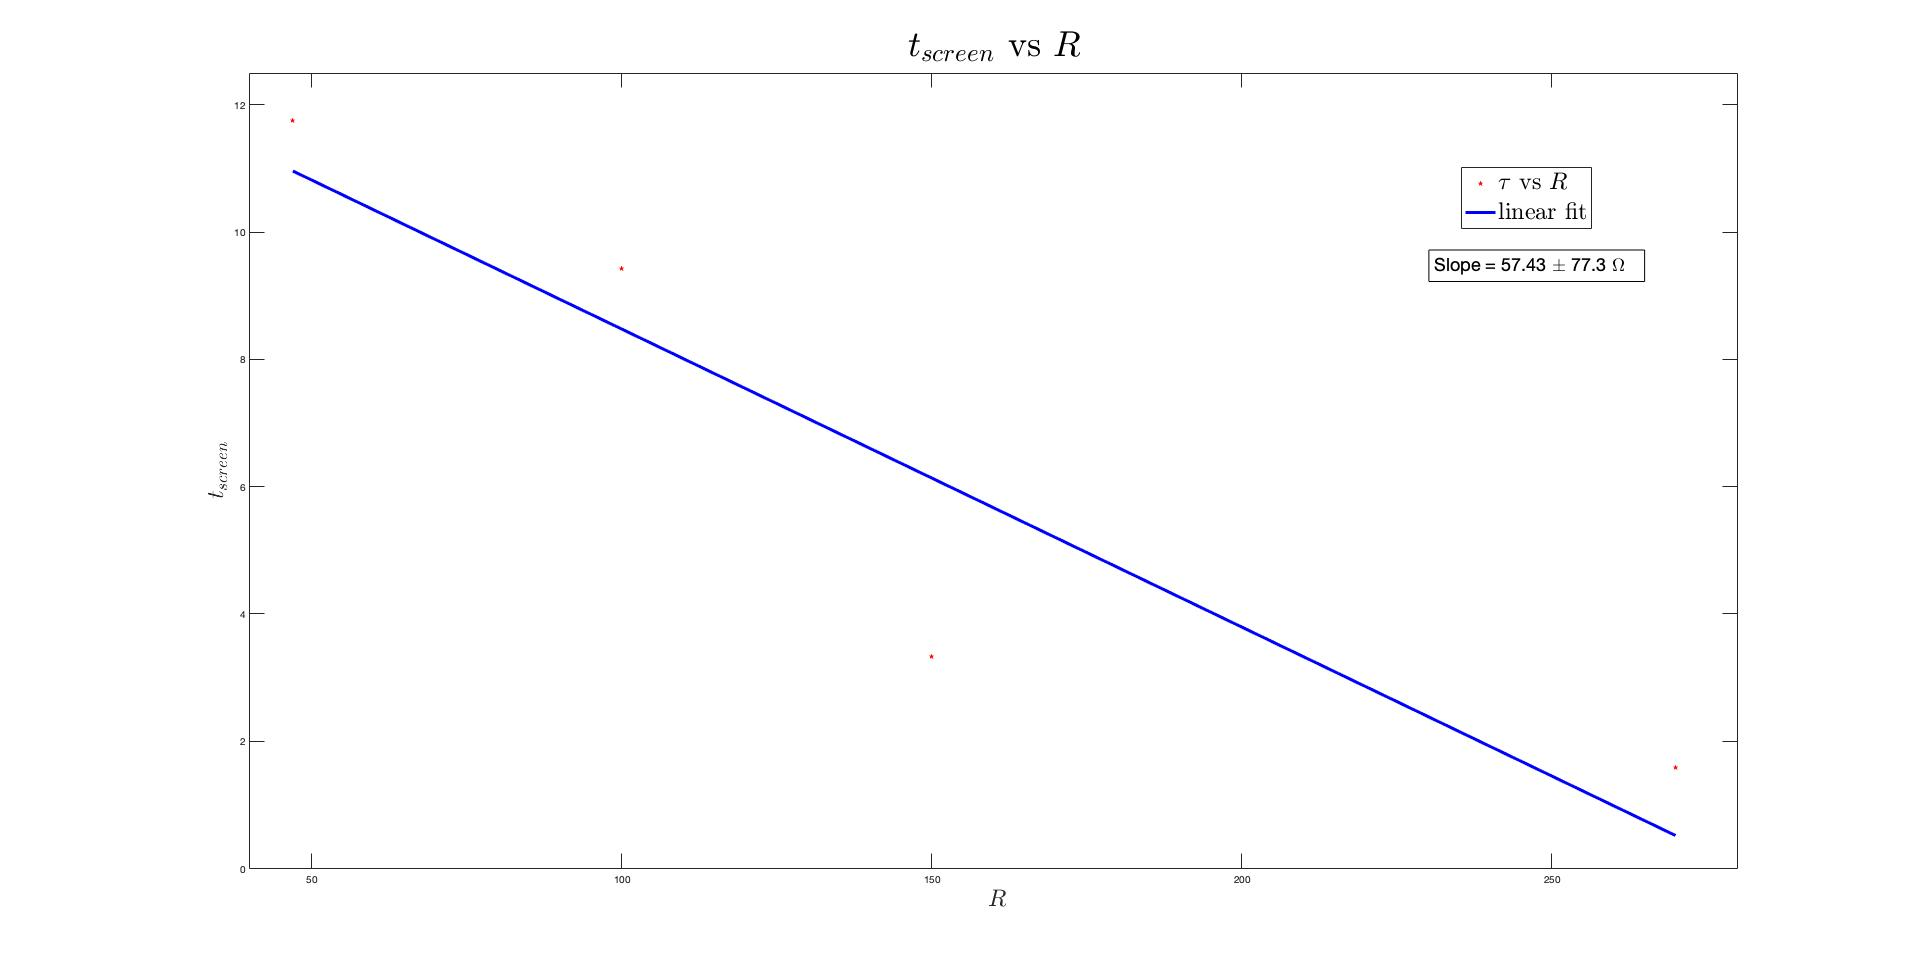
\includegraphics[width=\textwidth]{graph2.jpg}
\end{center}
\begin{itemize}
  \item What is the value of the slope in the second graph and how does that compare to what you expected?
  \item[] Slope = 57.43 \(\pm \) 77.3 \(\Omega \). I expected it to be bad since Sebastian said it would.
\end{itemize}
\end{document}
